\documentclass[11pt,a4paper]{article}
% FastForest — SoftwareX Original Software Publication, draft v0.1 (2026-10-17).
% Reading copy in the article class; move the body into Elsevier's elsarticle template (\journal{SoftwareX})
% at submission. Square-bracket red notes are for the authors.
\usepackage[utf8]{inputenc}
\usepackage[T1]{fontenc}
\IfFileExists{lmodern.sty}{\usepackage{lmodern}\usepackage{microtype}}{\usepackage[expansion=false]{microtype}}
\usepackage{textcomp}
\usepackage{amsmath,amssymb}
\usepackage[a4paper,margin=2.4cm]{geometry}
\usepackage{setspace}
\setstretch{1.1}
\usepackage{graphicx}
\usepackage{booktabs,longtable,array,multirow}
\newcolumntype{P}[1]{>{\raggedright\arraybackslash}p{#1}}
\usepackage[table]{xcolor}
\usepackage[font=small,labelfont=bf]{caption}
\usepackage{url}
\usepackage{listings}
\usepackage{tikz}
\usetikzlibrary{arrows.meta,positioning,shapes.misc}
\usepackage[colorlinks=true,linkcolor=blue!60!black,citecolor=blue!60!black,urlcolor=blue!60!black]{hyperref}
\definecolor{notecolor}{RGB}{170,60,20}
\newcommand{\authnote}[1]{{\color{notecolor}\small [#1]}}
\setlength{\parskip}{0.35em}
\setlength{\tabcolsep}{4pt}
\emergencystretch=2em
\lstset{basicstyle=\ttfamily\small,columns=fullflexible,keepspaces=true,frame=single,framerule=0.3pt,rulecolor=\color{gray!60},xleftmargin=0.6em,aboveskip=0.6em,belowskip=0.6em,breaklines=true}

\title{FastForest: random-forest feature reduction for high-dimensional tabular data}
\author{Tim O.\ Hulshof\textsuperscript{a,b}, Ines Thiele\textsuperscript{a,b,c,d}\\[0.6em]
\normalsize \textsuperscript{a} School of Medicine, University of Galway, Galway, Ireland \\
\normalsize \textsuperscript{b} Digital Metabolic Twin Centre, University of Galway, Galway, Ireland \\
\normalsize \textsuperscript{c} Ryan Institute, University of Galway, Galway, Ireland \\
\normalsize \textsuperscript{d} APC Microbiome Ireland, University College Cork, Cork, Ireland \\
\authnote{affiliations: harmonise with the synthetic-data paper}}
\date{Draft v0.1 — 17 October 2026 — for SoftwareX (Original Software Publication)}

\begin{document}
\maketitle

\noindent\authnote{Draft written from the Phase 3 benchmark (results/summary/, 484 comparison and 6 scalability runs, config hash 67e4df26de320349). SoftwareX asks for about 3,000 words in sections 1--5, the code-metadata table, and Elsevier's declarations; this reading copy uses the article class and will be moved into the elsarticle template at submission. The hosted app, the Zenodo DOI, the release version and the funding line are to be confirmed (red notes).}

\begin{abstract}
\noindent FastForest reduces a labelled table with thousands of columns to the few features a random forest needs to classify it, and reports how much accuracy that costs on data the selection never saw. It trains a forest on all features, ranks them by importance, searches over importance thresholds for the smallest subset whose validation accuracy stays within a user-set bound of the full model, removes redundant features by Spearman-correlation clustering, retrains, and evaluates once on a held-out test split. It is a Python library, a command-line tool and a web application. On ten tables of genome-scale metabolic reconstructions (up to 238,492 genomes $\times$ 5,844 reactions) and three public benchmarks, FastForest kept 2--11 times fewer features than Boruta, recursive feature elimination or L1-regularised logistic regression on the reaction-presence tables at equal or better accuracy, matched the accuracy of using every feature with 1.4\% of them or fewer on the public sets, and ran in seconds on 20,000-row tables and in 2--11 minutes on the full tables on a laptop. Its selected sets vary more between random splits than Boruta's, which the package reports as a stable core.
\end{abstract}

\noindent\textbf{Keywords:} random forest; feature selection; dimensionality reduction; tabular data; genome-scale metabolic reconstruction; Python

\begin{table}[htbp]
\small
\caption{Code metadata.}
\label{tab:metadata}
\begin{tabular}{P{0.6cm}P{6.2cm}P{8.6cm}}
\toprule
\textbf{Nr.} & \textbf{Code metadata description} & \\
\midrule
C1 & Current code version & 1.0.0 \authnote{1.0.0.dev0 on the repository today; tag the release before submission} \\
C2 & Permanent link to code/repository used for this code version & \url{https://github.com/ThieleLab/streamlit_random_forest_analysis} \authnote{add the Zenodo DOI of the tagged release} \\
C3 & Permanent link to reproducible capsule & \texttt{bash benchmarks/reproduce.sh} in the repository; Docker image built from the repository's \texttt{Dockerfile} \\
C4 & Legal code license & GPL-3.0-or-later \\
C5 & Code versioning system used & git \\
C6 & Software code languages, tools and services used & Python $\ge$ 3.10; NumPy, pandas, SciPy, scikit-learn, matplotlib, plotly, umap-learn; Streamlit (web app); Docker; GitHub Actions (CI) \\
C7 & Compilation requirements, operating environments and dependencies & Operating-system independent; \texttt{pip install} from the repository; no compiled extensions beyond the dependencies' wheels; tested on Python 3.10--3.12 \\
C8 & Link to developer documentation/manual & \texttt{README.md}, \texttt{CONTRIBUTING.md} and \texttt{benchmarks/README.md} in the repository; \texttt{fastforest reduce --help} \\
C9 & Support email for questions & t.hulshof1@universityofgalway.ie \\
\bottomrule
\end{tabular}
\end{table}

\section{Motivation and significance}

Many tables in computational biology have far more columns than a model needs. A genome-scale metabolic reconstruction describes an organism by the presence or abundance of several thousand reactions; a cohort of reconstructions is therefore a table with thousands of columns and a label per row, such as the taxon or the body site the genome was sampled from. The APOLLO resource holds 247,092 such reconstructions \cite{heinken2025}. Classifying such a table is not hard: a random forest on all columns reaches 99\% accuracy on the tables used here. What is hard is saying \emph{which} reactions carry the classification, because a forest grown on 5,000 features spreads its importance thinly and a biologist cannot interpret, validate or measure 5,000 of anything. The same situation arises with gene-expression, metabolomic and microbiome tables.

Feature selection is an old problem with many solutions, and the ones most used with forests answer slightly different questions. Boruta \cite{kursa2010} finds every feature that is more informative than its own shuffled copy, the \emph{all-relevant} set; recursive feature elimination with cross-validation (RFECV) \cite{guyon2002} removes features in steps and keeps the subset with the best cross-validated score; L1-regularised logistic regression \cite{tibshirani1996} keeps the features of a sparse linear model. None of them answers the question a user of a reconstruction table usually asks: \emph{what is the smallest set of features on which the classifier is as accurate as on all of them, within a tolerance I choose?} FastForest answers that question. It ranks features by random-forest importance, searches over importance thresholds for the smallest subset whose validation metrics stay within a bound of the full model, removes features that are near-duplicates of a more important one, and reports the final model on a test split that played no part in the selection. The bound is the only choice the user has to make, and it is stated in the units of the metric (the default allows a 0.05-percentage-point drop in accuracy).

An earlier, unpublished version of the method produced the taxonomic classifier of the APOLLO resource \cite{heinken2025}. This release rewrites it as a tested package with three interfaces (library, command line, web application), replaces the deep-learning preprocessing of the original with scikit-learn \cite{pedregosa2011}, and corrects two flaws of the original evaluation: the validation set is no longer used both to stop the threshold search and to report the result, and every random step is seeded. Section~\ref{sec:examples} benchmarks the release against Boruta, RFECV, a permutation-importance threshold and L1 logistic regression on ten reconstruction tables and three public feature-selection benchmarks, with ten or five random splits each, and times it on tables of up to 238,492 rows.

\section{Software description}

\subsection{Software architecture}

FastForest is a Python package, \texttt{fastforest}, with one estimator and one result object. \texttt{FastForest.fit(X, y)} takes a pandas table and a label column and returns a \texttt{FastForestResult} holding the selected features, the trained models, the importance ranking, the redundancy clusters, the metrics of every stage on the train, validation and test splits, the timings and the environment. The package has no dependency on the web framework; the Streamlit application (\texttt{app/streamlit\_app.py}) is a thin layer that calls the library and renders the figures it returns, and the command-line tool (\texttt{fastforest reduce}) writes the same result to disk as CSV and JSON. Figure~\ref{fig:pipeline} shows the stages; Table~\ref{tab:metadata} the metadata. The modules follow the stages: \texttt{preprocess}, \texttt{split}, \texttt{importance}, \texttt{reduce} (threshold search, redundancy, final model), \texttt{redundancy}, \texttt{metrics}, \texttt{result}, \texttt{viz}, \texttt{cli} and \texttt{datasets} (a bundled 1,000 $\times$ 500 subsample of the body-site table for examples and tests). The dependencies are NumPy, pandas, SciPy, scikit-learn, matplotlib, plotly and umap-learn; Streamlit is an optional extra. A test suite of 89 tests covers 99\% of the package's lines \authnote{recount at release} and runs in continuous integration on Python 3.10, 3.11 and 3.12; it includes a regression test for every defect found in the original implementation, among them the redundancy step that kept the alphabetically last member of a cluster instead of the most important one.

\begin{figure}[tbp]
\centering
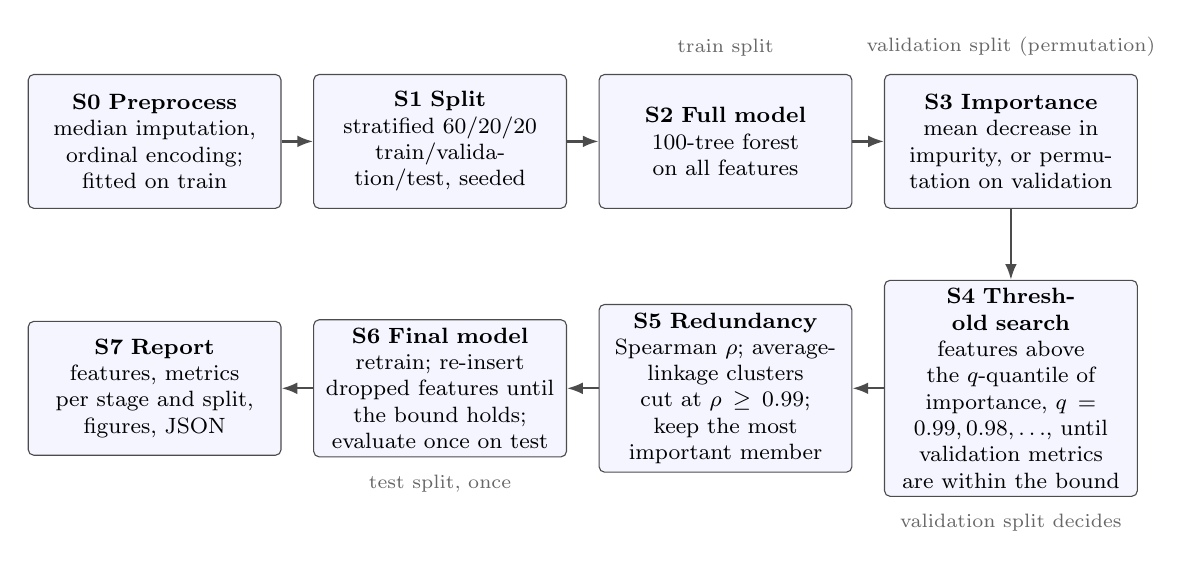
\begin{tikzpicture}[
  node distance=3mm and 4mm,
  stage/.style={draw=black!70, rounded corners=2pt, fill=blue!4, text width=3.0cm, align=center, font=\footnotesize, minimum height=1.7cm, inner sep=3pt},
  split/.style={draw=black!70, rounded corners=2pt, fill=orange!8, text width=2.0cm, align=center, font=\footnotesize, minimum height=0.8cm, inner sep=3pt},
  lab/.style={font=\scriptsize, text=black!60},
  arr/.style={-{Latex[length=2mm]}, thick, black!70}
]
\node[stage] (s0) {\textbf{S0 Preprocess}\\median imputation, ordinal encoding; fitted on train};
\node[stage, right=of s0] (s1) {\textbf{S1 Split}\\stratified 60/20/20 train/validation/test, seeded};
\node[stage, right=of s1] (s2) {\textbf{S2 Full model}\\100-tree forest on all features};
\node[stage, right=of s2] (s3) {\textbf{S3 Importance}\\mean decrease in impurity, or permutation on validation};
\node[stage, below=9mm of s3] (s4) {\textbf{S4 Threshold search}\\features above the $q$-quantile of importance, $q = 0.99, 0.98, \ldots$, until validation metrics are within the bound};
\node[stage, left=of s4] (s5) {\textbf{S5 Redundancy}\\Spearman $\rho$; average-linkage clusters cut at $\rho \ge 0.99$; keep the most important member};
\node[stage, left=of s5] (s6) {\textbf{S6 Final model}\\retrain; re-insert dropped features until the bound holds; evaluate once on test};
\node[stage, left=of s6] (s7) {\textbf{S7 Report}\\features, metrics per stage and split, figures, JSON};
\draw[arr] (s0) -- (s1); \draw[arr] (s1) -- (s2); \draw[arr] (s2) -- (s3);
\draw[arr] (s3) -- (s4); \draw[arr] (s4) -- (s5); \draw[arr] (s5) -- (s6); \draw[arr] (s6) -- (s7);
\node[lab, above=1mm of s2] {train split};
\node[lab, above=1mm of s3] {validation split (permutation)};
\node[lab, below=1mm of s4] {validation split decides};
\node[lab, below=1mm of s6] {test split, once};
\end{tikzpicture}
\caption{The FastForest pipeline. Decisions (the stopping threshold and the re-insertion of features after redundancy removal) use the validation split only; the test split is evaluated once, by the final model.}
\label{fig:pipeline}
\end{figure}

\subsection{Software functionalities}

\emph{Input.} A CSV, TSV or Parquet table with one class column; numeric and categorical columns are accepted. Missing numeric values are median-imputed and categorical columns ordinal-encoded, with the encoders fitted on the training split only. Values are not scaled, because trees are invariant to monotone transformations and unscaled histograms are easier to read.

\emph{Splits.} The rows are split, stratified by class, into training, validation and test sets (60/20/20 by default). The forest is trained on the training split; the threshold search and the bound are decided on the validation split; the test split is touched once, by the final model. A caller can pass its own split indices, so that several methods can be compared on identical splits, or name the rows that must form the test set.

\emph{Importance and threshold search.} A random forest with 100 trees, half of the features considered at each split and at least five samples per leaf is trained on all features, and features are ranked by mean decrease in impurity \cite{louppe2013} or, optionally, by permutation importance measured on the validation split. The search keeps the features whose importance exceeds the $q$-quantile of the positive importances, for $q = 0.99, 0.98, \ldots, 0$, retrains at each step and stops at the first $q$ for which the validation metrics are within the bound of the full model. The bound applies to accuracy, or to accuracy, macro precision and macro recall together. If no threshold satisfies the bound, all features with positive importance are kept and the fact is reported.

\emph{Redundancy removal.} Among the kept features, pairs with Spearman correlation of at least 0.99 (a cut at $1 - \rho = 0.01$ in an average-linkage dendrogram) are merged and the most important member of each cluster is kept. Reaction tables contain many such pairs: reactions of one pathway are present or absent together.

\emph{Final model and bound enforcement.} The forest is retrained on the remaining features. If the validation metrics now fall outside the bound, the features removed as redundant are re-inserted in order of importance until it holds. The final model is evaluated on the test split.

\emph{Outputs.} The selected features in importance order; accuracy, macro precision, recall and F1 for every stage on every split; the full importance ranking; the clusters; the timings of every stage; the parameters and the software versions, so that a run can be repeated from its JSON. Figures: confusion matrices, the importance bar chart, the threshold-search curve, the redundancy dendrogram, per-class heatmaps and histograms of the selected features, and linear-discriminant and UMAP \cite{mcinnes2018} projections of the reduced table.

\emph{Interfaces.} The library exposes the estimator and the figures as matplotlib and plotly objects. The command line, \texttt{fastforest reduce table.csv --target Class --out dir}, writes \texttt{features.csv}, \texttt{metrics.json}, \texttt{importances.csv}, \texttt{clusters.json} and the figures. The web application lets a user upload a table or pick the bundled sample, choose the class column, bound, seed, importance measure and redundancy cut, run the pipeline with a progress bar, inspect every stage and download the feature list; it is hosted at \url{https://fastforest.vmh.life} \authnote{confirm the hosted instance is running at submission} and runs locally with one command or with Docker.

\subsection{Sample code}

\begin{lstlisting}[language=Python]
from fastforest import FastForest, load_sample, viz

X, y = load_sample()                       # 1,000 genomes x 500 reactions, 4 body sites
result = FastForest(bound=5e-4, criterion="accuracy",
                    n_estimators=100, random_state=0).fit(X, y)
result.features_final                      # selected features, most important first
result.metrics["final"]["test"]            # accuracy and macro precision / recall / F1
result.summary()                           # one row per stage and split
viz.dendrogram(result.redundancy).savefig("dendrogram.png")
result.to_json("fastforest_result.json")   # parameters, metrics, timings, environment
\end{lstlisting}

\noindent The same run from a shell: \texttt{fastforest reduce reaction\_abundance\_body\_site.csv --target "Body site" --out results/demo --seed 0}.

\section{Illustrative examples}
\label{sec:examples}

\subsection{Reducing a reaction-abundance table}

The repository ships the table that motivated the tool: 1,957 APOLLO genomes with the abundance of 8,306 reactions, labelled with four body sites. With the default bound, FastForest keeps 27 reactions on average over ten random splits (standard deviation 18) and the final model classifies the test split with 99.18 $\pm$ 0.60\% accuracy, against 99.16 $\pm$ 0.51\% for a forest on all 8,306 reactions; the whole run takes 6~s on a laptop. The application shows, stage by stage, where the accuracy goes: the threshold search stops at $q$ between 0.76 and 0.95 (0.90--0.95 in eight of the ten seeds), the redundancy step removes a further one to twelve reactions, and the bound held in every run. A random subset of 27 reactions, the control that shows the selection is not trivial, reaches 96.60 $\pm$ 0.90\%.

\subsection{Comparison with other selection methods}

We compared FastForest with Boruta \cite{kursa2010}, RFECV \cite{guyon2002}, a permutation-importance threshold (keep every feature whose permutation importance on the validation split is positive), L1-regularised logistic regression \cite{tibshirani1996}, and two controls: no selection and a random subset of the size FastForest chose on the same split. The benchmark harness, its configuration and all per-run results are in the repository (\texttt{benchmarks/}, \texttt{results/summary/}); \texttt{bash benchmarks/reproduce.sh} regenerates every table and figure of this section.

\emph{Data.} Ten tables of reconstruction data and three public benchmarks (Table~\ref{tab:datasets}). The reaction-presence tables come from APOLLO \cite{heinken2025}: binary presence of 5,129--5,844 reactions in 51,884--238,492 reconstructions, labelled with phylum, order or genus, for the combined resource and for its two halves (sequenced genomes and gut metagenome-assembled genomes). The public sets are Madelon and Gisette from the NIPS 2003 feature-selection challenge \cite{guyon2004}, whose features are known to be real or random probes, and the GEMLeR breast-versus-rest gene-expression table \cite{stiglic2010}, all from OpenML. Classes with fewer than ten rows were dropped, and tables with more than 20,000 rows were stratified-subsampled once to 20,000 rows for the comparison; FastForest alone was also run on the full rows (Section~\ref{sec:scalability}).

\begin{table}[tbp]
\small
\caption{Datasets. Rows are those used in the comparison, with the full table's rows in parentheses where it was subsampled to 20,000; classes are those with at least ten rows after subsampling. The six half tables (sequenced genomes and gut MAGs at phylum, order and genus level) were run with one seed and are shown in Supplementary Fig.~S1.}
\label{tab:datasets}
\begin{tabular}{P{4.6cm}P{3.4cm}rrrl}
\toprule
\textbf{Table} & \textbf{Source} & \textbf{Rows} & \textbf{Features} & \textbf{Classes} & \textbf{Seeds} \\
\midrule
Reaction abundance, body site & APOLLO (bundled) & 1,957 & 8,306 & 4 & 10 \\
Reaction presence, combined, phylum & APOLLO \cite{heinken2025} & 19,982 (238,492) & 5,129 & 11 & 5 \\
Reaction presence, combined, order & APOLLO & 19,918 (237,337) & 5,129 & 39 & 5 \\
Reaction presence, combined, genus & APOLLO & 19,730 (181,628) & 5,129 & 105 & 5 \\
Madelon & NIPS 2003, OpenML 1485 & 2,600 & 500 & 2 & 10 \\
Gisette & NIPS 2003, OpenML 41026 & 7,000 & 5,000 & 2 & 10 \\
GEMLeR breast vs rest & OpenML 1128 & 1,545 & 10,935 & 2 & 10 \\
\bottomrule
\end{tabular}
\end{table}

\emph{Protocol.} For every table and seed, the rows were split 60/20/20 and the split shared by every method. Each method selected features on the training split, plus the validation split where it needs one (FastForest's threshold search, the permutation threshold). A fresh 100-tree forest with FastForest's hyper-parameters was then trained on the training rows of the selected features and evaluated once on the test split, so that every method is judged by the same classifier on the same rows. Boruta ran with the same 100-tree forest and kept confirmed features only; RFECV removed 10\% of the features per step with five-fold cross-validation on the training split; the L1 model used one-versus-rest liblinear fits with the regularisation chosen by five-fold cross-validation under the one-standard-error rule, because the cross-validation optimum kept 8,158 of the 8,306 body-site features. The body-site table and the three public sets ran ten seeds, the three combined APOLLO tables five, their halves one; the L1 baseline at genus level (105 one-versus-rest fits, 78~min per run) was run once. In all, 484 comparison runs completed without failure.

\emph{Reduction and accuracy.} Table~\ref{tab:results} and Fig.~\ref{fig:reduction} give the result. On the reaction-presence tables FastForest kept 2--11 times fewer features than Boruta, RFECV or L1 logistic regression at equal or better accuracy, and on the body-site table 3--150 times fewer: 145 of 5,129 reactions at phylum level (99.49\% against 99.45\% with every reaction), 265 at order level (97.58\%, the best of all methods on this 39-class task, against 97.07\% with every reaction) and 699 at genus level (97.52\% against 97.58\%). On the body-site table it kept 27 of 8,306 reactions at 99.18\%. On the public benchmarks it matched or exceeded the accuracy of using every feature while keeping 1.4\% of them or fewer (7 of 500 on Madelon, 89 of 5,000 on Gisette, 12 of 10,935 on GEMLeR), but the best baseline was 0.4--1.8 percentage points more accurate with 3--12 times more features: Boruta on Madelon (86.23\% with 21 features against 84.48\% with 7), RFECV on Gisette (96.59\% with 850 against 96.20\% with 89) and L1 on GEMLeR (96.50\% with 155 against 96.08\% with 12, within one standard deviation). This is the trade-off the method is built around: it stops at the smallest set that satisfies the bound on the validation split, not at the most accurate set. The random-subset control lost 2--34 points everywhere, so the sets are not trivial. FastForest with permutation importance kept fewer features still but was unreliable on the small body-site table (91.4 $\pm$ 10.3\%), because few features there have positive permutation importance and the search cannot meet the bound within them; the default, impurity importance, is the one to use.

\begin{table}[tbp]
\small
\caption{Features kept (mean over seeds), test accuracy (\%, mean $\pm$ SD over seeds) of a 100-tree random forest trained on each method's selection, and selection time. ``All'' is the forest on every feature and ``Random'' a random subset of FastForest's size. Selection time is the mean wall-clock time of the selection step on an Apple M2 Pro laptop, measured at low process priority while the machine was in use, so the times are indicative. L1 at genus level is a single run.}
\label{tab:results}
\setlength{\tabcolsep}{3pt}
\begin{tabular}{P{3.1cm}rrrrrr}
\toprule
\textbf{Table} & \textbf{FastForest} & \textbf{Boruta} & \textbf{RFECV} & \textbf{L1 logistic} & \textbf{All} & \textbf{Random} \\
\midrule
\multicolumn{7}{l}{\emph{Features kept}} \\
Body site & 27 & 83 & 4,156 & 533 & 8,306 & 27 \\
Combined, phylum & 145 & 570 & 931 & 1,558 & 5,129 & 145 \\
Combined, order & 265 & 676 & 1,033 & 2,923 & 5,129 & 265 \\
Combined, genus & 699 & 1,397 & 2,467 & 3,226 & 5,129 & 699 \\
Madelon & 7 & 21 & 50 & 1 & 500 & 7 \\
Gisette & 89 & 229 & 850 & 601 & 5,000 & 89 \\
GEMLeR breast & 12 & 55 & 4,596 & 155 & 10,935 & 12 \\
\midrule
\multicolumn{7}{l}{\emph{Test accuracy, \%}} \\
Body site & 99.18 $\pm$ 0.60 & 99.08 $\pm$ 0.39 & 99.10 $\pm$ 0.53 & 98.93 $\pm$ 0.67 & 99.16 $\pm$ 0.51 & 96.60 $\pm$ 0.90 \\
Combined, phylum & 99.49 $\pm$ 0.08 & 99.43 $\pm$ 0.14 & 99.46 $\pm$ 0.17 & 99.44 $\pm$ 0.14 & 99.45 $\pm$ 0.10 & 97.30 $\pm$ 0.81 \\
Combined, order & 97.58 $\pm$ 0.24 & 97.09 $\pm$ 0.40 & 97.10 $\pm$ 0.51 & 97.08 $\pm$ 0.37 & 97.07 $\pm$ 0.41 & 94.19 $\pm$ 0.53 \\
Combined, genus & 97.52 $\pm$ 0.17 & 97.60 $\pm$ 0.26 & 97.56 $\pm$ 0.25 & 97.49 & 97.58 $\pm$ 0.18 & 95.19 $\pm$ 0.89 \\
Madelon & 84.48 $\pm$ 2.63 & 86.23 $\pm$ 1.35 & 83.77 $\pm$ 1.87 & 55.87 $\pm$ 2.10 & 80.38 $\pm$ 1.86 & 50.58 $\pm$ 1.14 \\
Gisette & 96.20 $\pm$ 0.29 & 96.49 $\pm$ 0.35 & 96.59 $\pm$ 0.37 & 96.50 $\pm$ 0.32 & 96.11 $\pm$ 0.46 & 87.61 $\pm$ 3.45 \\
GEMLeR breast & 96.08 $\pm$ 1.10 & 96.41 $\pm$ 1.12 & 96.05 $\pm$ 1.23 & 96.50 $\pm$ 0.89 & 96.02 $\pm$ 1.39 & 81.72 $\pm$ 4.70 \\
\midrule
\multicolumn{7}{l}{\emph{Selection time, s}} \\
Body site & 6 & 70 & 76 & 6 & -- & -- \\
Combined, phylum & 23 & 936 & 330 & 461 & -- & -- \\
Combined, order & 27 & 951 & 335 & 1,823 & -- & -- \\
Combined, genus & 98 & 1,568 & 381 & 4,677 & -- & -- \\
Madelon & 1.5 & 23 & 30 & 1.9 & -- & -- \\
Gisette & 13 & 303 & 250 & 7 & -- & -- \\
GEMLeR breast & 13 & 203 & 270 & 4 & -- & -- \\
\bottomrule
\end{tabular}
\end{table}

\begin{figure}[tbp]
\centering
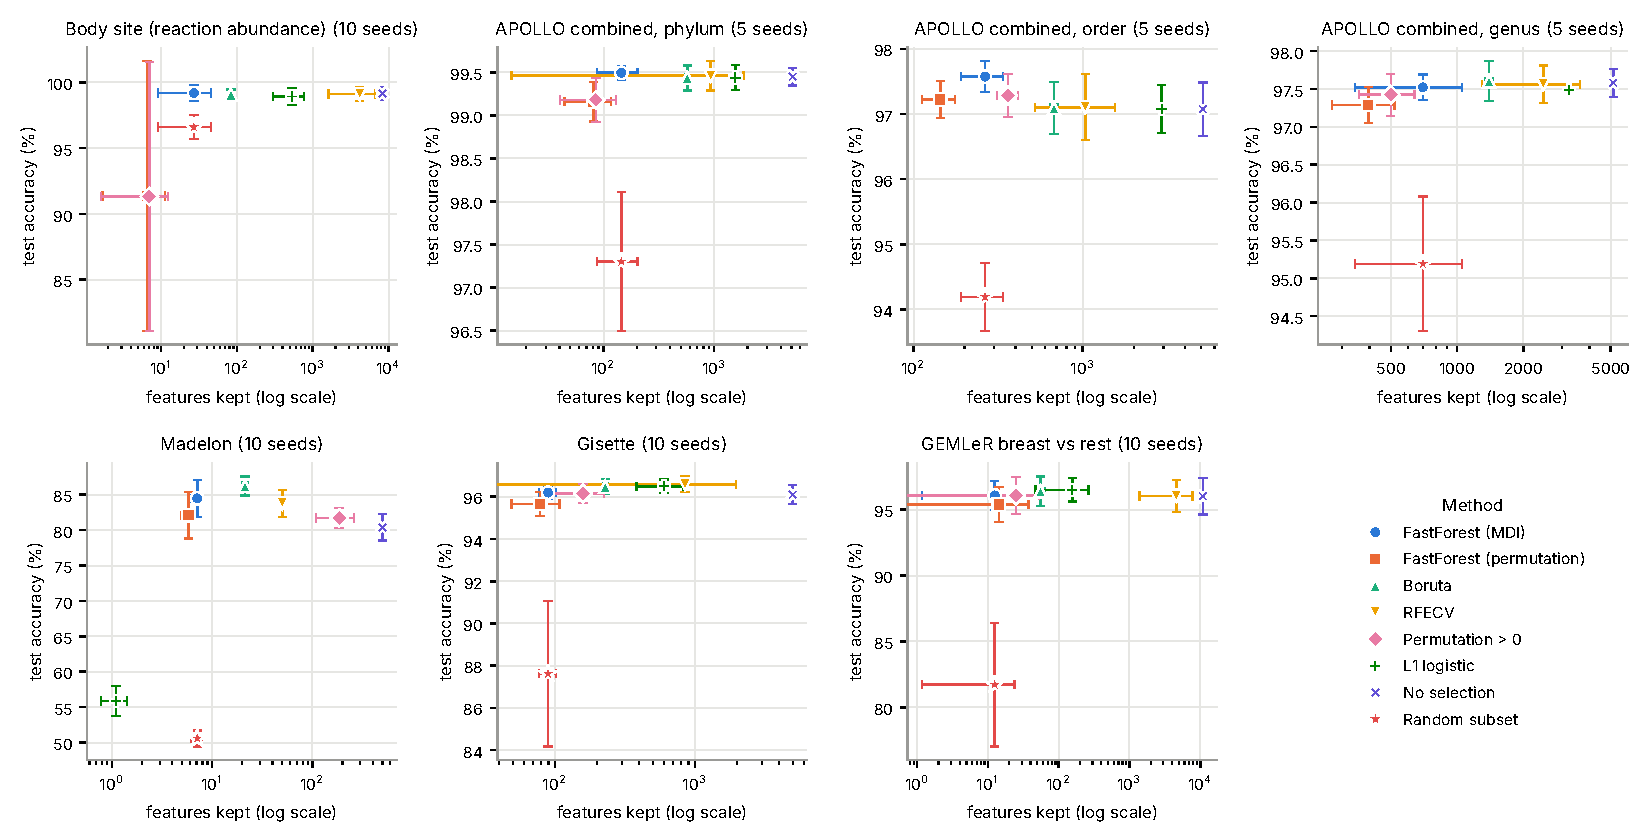
\includegraphics[width=\textwidth]{figures/fig2_reduction_vs_accuracy.pdf}
\caption{Features kept against test accuracy for every method on the seven tables with repeated splits (mean $\pm$ SD over seeds; the number of features on a log scale). FastForest sits at the left edge of every panel at the accuracy of the full model; on the public benchmarks one baseline is slightly more accurate with many more features. The six single-seed half tables are in Supplementary Fig.~S1.}
\label{fig:reduction}
\end{figure}

\emph{Time.} FastForest's selection took 1.5--98~s on the 20,000-row tables (Table~\ref{tab:results}), against 23~s to 26~min for Boruta, 30~s to 6~min for RFECV and 2~s to 78~min for the L1 model, whose cost grows with the number of classes. Most of FastForest's time is the initial forest; the threshold search retrains on a shrinking set and is cheap by comparison.

\emph{Stability.} How much a selected set changes between random splits matters when the features are to be interpreted. Measured as the mean pairwise Jaccard similarity of the sets selected under different seeds (Fig.~\ref{fig:stability}), FastForest is less stable than Boruta on the combined APOLLO tables (0.39--0.48 against 0.69--0.85) and on Gisette (0.47 against 0.61), comparable on the body-site table (0.43 against 0.47) and on GEMLeR (0.43 against 0.35), and high on Madelon (0.77). This is the expected cost of asking for a minimal sufficient set rather than an all-relevant one: when several reactions carry the same information, which of them survives the threshold depends on the split. For that reason the package reports, alongside each run, the size of the selected set across seeds, and the benchmark records the \emph{core}---the features selected under every seed---which on the combined APOLLO tables holds 48 of the 145 phylum-level reactions, 113 of 265 at order level and 274 of 699 at genus level. Users who need a stable list should run several seeds and take the core, or use Boruta where the all-relevant set is wanted \authnote{Tim: this is the answer proposed to the open question on stability; a stability-selection option in the package would be the alternative}.

\begin{figure}[tbp]
\centering
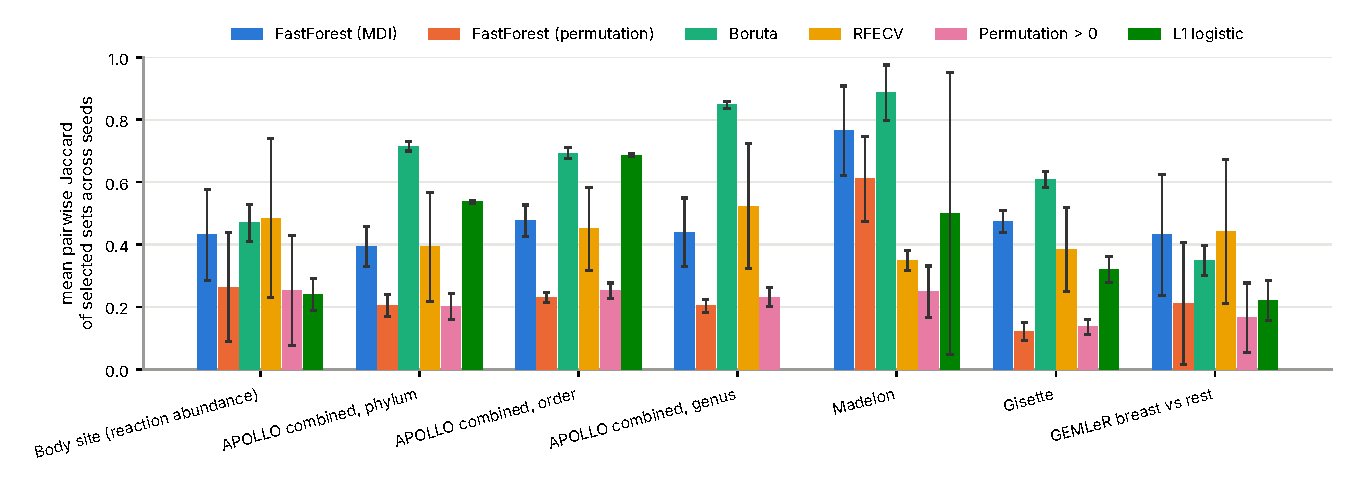
\includegraphics[width=\textwidth]{figures/fig3_stability.pdf}
\caption{Stability of the selected sets: mean pairwise Jaccard similarity across seeds (error bars $\pm$ SD over pairs). The no-selection control is 1 by definition and the random control below 0.07; both are omitted. L1 at genus level has one run.}
\label{fig:stability}
\end{figure}

\emph{Recovering known features.} Madelon has 20 relevant features---5 informative ones and 15 linear combinations of them---among 480 random probes; the identities are not published but follow from the documented construction, and exactly 20 features of the OpenML table are correlated with another feature while every probe is not. FastForest's selection was always made of relevant features (precision 1.00 over ten seeds) but kept about 7 of the 20 (recall 0.35), a sufficient set given that 15 of the 20 are combinations of the other 5; Boruta recovered 19.9 of 20 with precision 0.94, RFECV all 20 among 50 kept, the L1 model one, and the permutation threshold 18 among 185 (Fig.~\ref{fig:recovery}). Gisette's probes cannot be told from its real features by the same test, so it has no recovery score. The example makes the difference between the methods concrete: Boruta returns everything that is relevant; FastForest returns what suffices.

\begin{figure}[tbp]
\centering
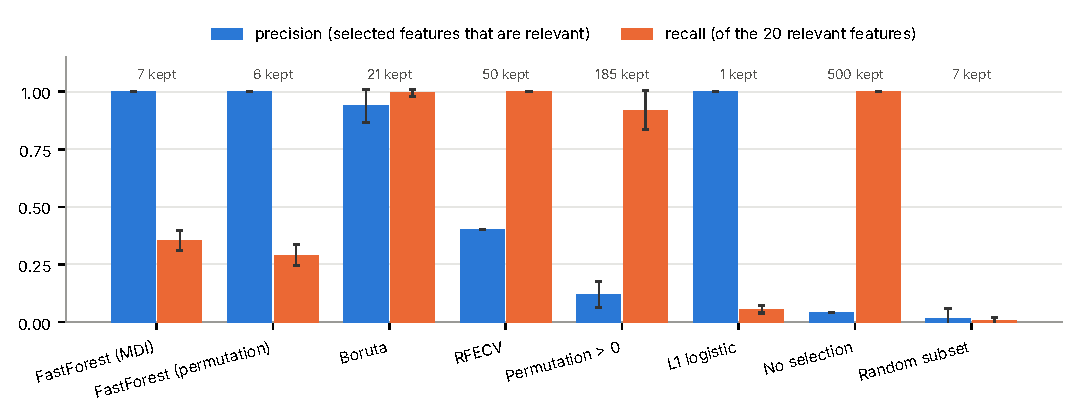
\includegraphics[width=0.9\textwidth]{figures/fig4_madelon_recovery.pdf}
\caption{Recovery of the 20 relevant features of Madelon over ten seeds: precision (fraction of the selected features that are relevant) and recall (fraction of the 20 that were selected), with the mean number of features kept above each pair of bars.}
\label{fig:recovery}
\end{figure}

\subsection{Scalability}
\label{sec:scalability}

FastForest with its defaults was run on the six full reaction-presence tables on an otherwise idle laptop (Apple M2 Pro, 10 cores, 16~GB; Table~\ref{tab:scalability}). The combined phylum table, 238,492 genomes $\times$ 5,129 reactions, was reduced to 108 reactions in 9.1~min at 99.84\% test accuracy, the 59-class order table to 341 reactions in 11.0~min at 99.28\%; the smaller tables took 1.7--5.1~min. Peak memory stayed below 4~GB. The initial forest took 84--502~s of each run, the threshold search 9--195~s and the final model under 30~s, so the cost is close to that of training one forest on the full table.

\begin{table}[tbp]
\small
\caption{FastForest on the full reaction-presence tables (default parameters, seed 0, idle laptop). ``Kept'' is the number of reactions in the final model.}
\label{tab:scalability}
\begin{tabular}{P{3.8cm}rrrrrrr}
\toprule
\textbf{Table} & \textbf{Rows} & \textbf{Features} & \textbf{Classes} & \textbf{Kept} & \textbf{Test acc.\ \%} & \textbf{Minutes} & \textbf{Peak GB} \\
\midrule
Combined, phylum & 238,492 & 5,129 & 14 & 108 & 99.84 & 9.1 & 3.7 \\
Combined, order & 237,337 & 5,129 & 59 & 341 & 99.28 & 11.0 & 3.8 \\
Sequenced genomes, phylum & 147,022 & 5,844 & 14 & 139 & 99.88 & 4.5 & 3.7 \\
Sequenced genomes, order & 146,997 & 5,844 & 51 & 329 & 99.29 & 5.1 & 3.8 \\
Gut MAGs, phylum & 91,470 & 5,374 & 9 & 122 & 99.86 & 2.2 & 2.9 \\
Gut MAGs, order & 90,327 & 5,374 & 25 & 106 & 99.75 & 1.7 & 2.7 \\
\bottomrule
\end{tabular}
\end{table}

\section{Impact}

FastForest turns a table with thousands of columns into a short, ranked list of the columns that classify it, with an honest estimate of what the reduction costs, in the time it takes to train one forest. In our own work the method produced the taxonomic classifier of the APOLLO resource \cite{heinken2025}, where a few hundred reactions out of five thousand reproduce the taxonomy of a quarter of a million reconstructions; the reduced reaction sets are the starting point for asking which metabolic capabilities define a taxon or a body site, a question that a 5,000-feature forest cannot answer. The benchmark here shows the same behaviour on gene-expression and synthetic data, so the tool applies to any labelled table with more columns than a person can read.

Three properties make it usable beyond its origin. It is fast enough to be run repeatedly---across seeds, bounds or label columns---on a laptop, which the comparison methods are not on tables of this size. It separates the decision from the report: the validation split chooses, the test split judges, and the result records both, so a user can quote the test accuracy of the reduced model without the optimism that a single split used for both would give. And it has three interfaces for three kinds of user: the web application for someone with a spreadsheet and no Python, the command line for a pipeline, the library for a notebook, all producing the same result object. The benchmark harness is part of the repository and reproduces every number in this paper with one command, which also makes it a template for comparing a new selection method on the same tables and splits.

The method's limits are stated by its results. It finds a sufficient set, not the all-relevant set, so it is the wrong tool when every informative feature is wanted; its sets are less stable than Boruta's across splits, which the core-feature report mitigates but does not remove; the bound is enforced on the validation split, so on very small tables the test accuracy can still differ from it; and the permutation-importance variant should be used only on tables with enough rows for the importances to be positive for the relevant features.

\section{Conclusions}

FastForest is a small, tested and reproducible implementation of one idea: keep the fewest features for which a random forest is as accurate as on all of them, within a bound the user sets, and say so on data the selection never saw. On thirteen tables it kept between 0.1\% and 14\% of the features at the accuracy of the full model, 2--11 times fewer than established methods on the reaction-presence tables, and met its validation bound in every one of the 484 benchmark runs, in seconds on 20,000-row tables and minutes on tables of a quarter of a million rows. It is available as a Python package, a command-line tool and a web application under the GPL-3.0 licence.

\section*{Declaration of competing interest}
The authors declare that they have no known competing financial interests or personal relationships that could have appeared to influence the work reported in this paper.

\section*{CRediT authorship contribution statement}
\textbf{Tim O.\ Hulshof:} Conceptualisation, Methodology, Software, Validation, Investigation, Data curation, Writing -- original draft, Visualisation. \textbf{Ines Thiele:} Conceptualisation, Resources, Supervision, Funding acquisition, Writing -- review and editing. \authnote{confirm}

\section*{Declaration of generative AI and AI-assisted technologies in the writing process}
During the preparation of this work the authors used Claude (Anthropic) to draft parts of the software, the benchmark code and the manuscript text under their direction. After using this tool, the authors reviewed, tested and edited the content and take full responsibility for the content of the publication. \authnote{Elsevier's required wording; adjust to taste}

\section*{Data availability}
The body-site table ships with the software. The reaction-presence tables were derived from the APOLLO reconstructions \cite{heinken2025} \authnote{state where the prepared tables are deposited (Zenodo) or how to rebuild them from APOLLO}; Madelon, Gisette and GEMLeR were obtained from OpenML (data sets 1485, 41026 and 1128). All per-run results, summary tables and figures of this paper are in the repository under \texttt{results/summary/} and are regenerated by \texttt{bash benchmarks/reproduce.sh}.

\section*{Acknowledgements}
\authnote{Funding: the earlier manuscript cited ERC grant 757922; the RECON4IMD (Horizon Europe) grant number is with Ines. Add the APOLLO co-authors' data contribution if required.}

\section*{References}
\noindent\authnote{Draft reference list: check every entry against CrossRef before submission, as for the synthetic-data paper.}
\renewcommand{\refname}{}
\begin{thebibliography}{99}
\vspace{-2.5em}

\bibitem{heinken2025} Heinken A, Hulshof TO, et al. APOLLO: a genome-scale metabolic reconstruction resource of 247,092 diverse human microbes spanning multiple continents, age groups, and body sites. Cell Syst 2025. doi:10.1016/j.cels.2025.101196 \authnote{complete the author list, volume and article number}
\bibitem{kursa2010} Kursa MB, Rudnicki WR. Feature selection with the Boruta package. J Stat Softw 2010;36(11):1--13. doi:10.18637/jss.v036.i11
\bibitem{guyon2002} Guyon I, Weston J, Barnhill S, Vapnik V. Gene selection for cancer classification using support vector machines. Mach Learn 2002;46:389--422. doi:10.1023/A:1012487302797
\bibitem{tibshirani1996} Tibshirani R. Regression shrinkage and selection via the lasso. J R Stat Soc B 1996;58:267--288.
\bibitem{pedregosa2011} Pedregosa F, Varoquaux G, Gramfort A, et al. Scikit-learn: machine learning in Python. J Mach Learn Res 2011;12:2825--2830.
\bibitem{breiman2001} Breiman L. Random forests. Mach Learn 2001;45:5--32. doi:10.1023/A:1010933404324
\bibitem{louppe2013} Louppe G, Wehenkel L, Sutera A, Geurts P. Understanding variable importances in forests of randomized trees. Adv Neural Inf Process Syst 2013;26:431--439.
\bibitem{mcinnes2018} McInnes L, Healy J, Saul N, Gro{\ss}berger L. UMAP: uniform manifold approximation and projection. J Open Source Softw 2018;3(29):861. doi:10.21105/joss.00861
\bibitem{guyon2004} Guyon I, Gunn S, Ben-Hur A, Dror G. Result analysis of the NIPS 2003 feature selection challenge. Adv Neural Inf Process Syst 2004;17:545--552.
\bibitem{stiglic2010} Stiglic G, Kokol P. Stability of ranked gene lists in large microarray analysis studies. J Biomed Biotechnol 2010;2010:616358. doi:10.1155/2010/616358
\bibitem{kalousis2007} Kalousis A, Prados J, Hilario M. Stability of feature selection algorithms: a study on high-dimensional spaces. Knowl Inf Syst 2007;12:95--116. doi:10.1007/s10115-006-0040-8
\end{thebibliography}

\clearpage
\section*{Supplementary material}
\renewcommand{\thefigure}{S\arabic{figure}}\setcounter{figure}{0}
\begin{figure}[htbp]
\centering
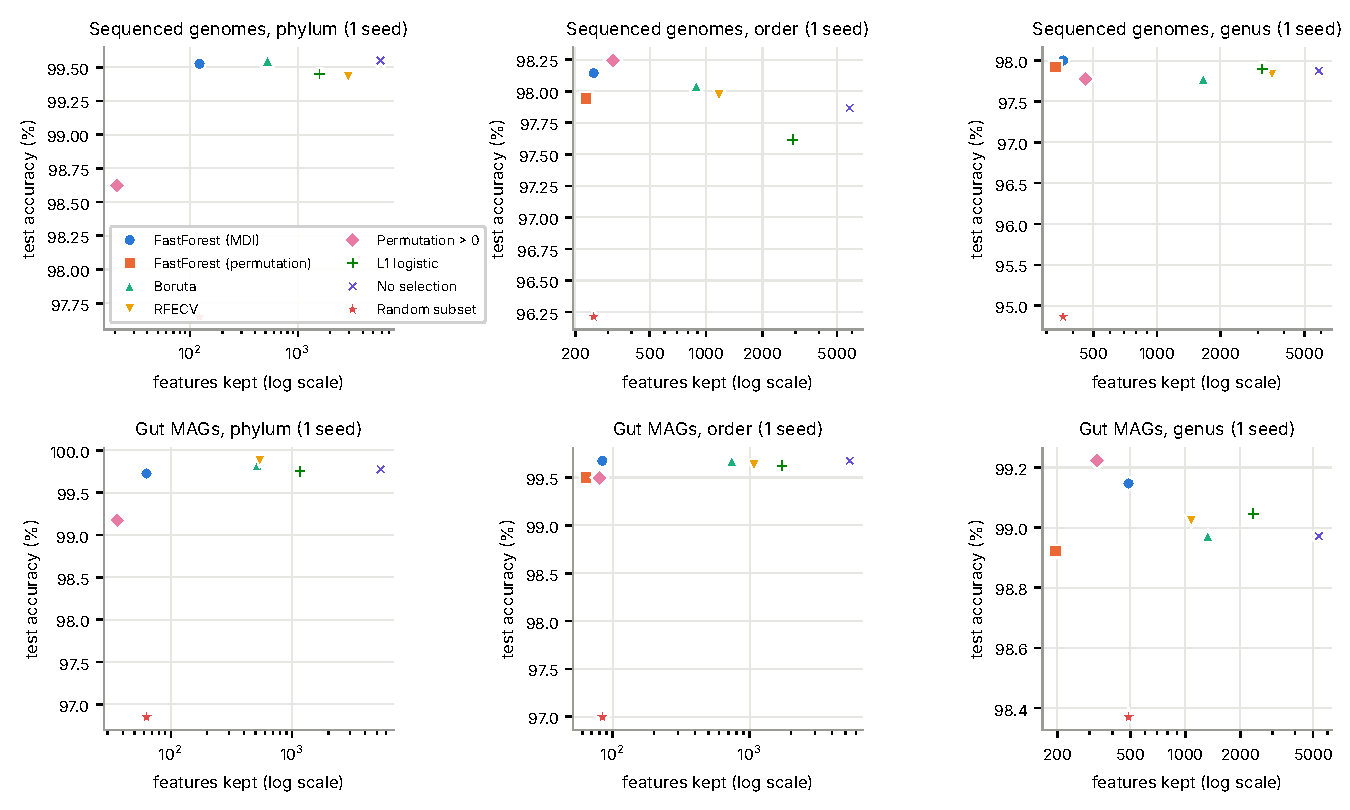
\includegraphics[width=\textwidth]{figures/figS1_half_tables.pdf}
\caption{Features kept against test accuracy on the six half tables of the APOLLO resource (sequenced genomes and gut metagenome-assembled genomes at phylum, order and genus level; 20,000-row subsamples, one seed each). The pattern of Fig.~2 repeats: FastForest at the left edge at the accuracy of the full model.}
\end{figure}

\end{document}
